\documentclass[10pt]{article}
% Transactions on Machine Learning Research (TMLR) Style
% Use \usepackage{tmlr} for anonymous submission to OpenReview
% Use \usepackage[preprint]{tmlr} for arXiv preprints
% Use \usepackage[accepted]{tmlr} for camera-ready publication
\usepackage{tmlr}

\usepackage{amsmath,amssymb,amsfonts,amsthm,bm}
\usepackage{graphicx}
\usepackage{booktabs}
\usepackage{tabularx}
\usepackage{multirow}
\usepackage{url}
\usepackage{hyperref}
\hypersetup{hidelinks}
\usepackage{color}
\usepackage{subcaption}
\usepackage{microtype}

\newcommand{\E}{\mathbb{E}}
\newcommand{\R}{\mathbb{R}}
\newcommand{\loss}{\mathcal{L}}
\newcommand{\dataset}{\mathcal{D}}
\newcommand{\EffRank}{\mathrm{EffRank}}
\newcommand{\Dcka}{D_{\mathrm{CKA}}}
\newcommand{\vtheta}{\bm{\theta}}
\newcommand{\urec}{u_{\mathrm{rec}}}

\title{Supplementary Material for:\\
Transient Collapse and Asymptotic Plasticity: How Procedural Resets Confound Auxiliary Transfer in Deep Vision}

\author{\name Vishesh Panghal \email pvt.panghal@gmail.com \\
      \addr Department of Artificial Intelligence and Data Science\\
      Poornima Institute of Engineering and Technology, Jaipur, India
      \AND
      \name Lakhan Bhaskar Kadel \email Lbhaskar@iujaipur.edu.in \\
      \addr Department of Computer Science and Engineering\\
      The ICFAI University, Jaipur, India
      \AND
      \name Shalini Pathak \email shalini.pathak@jaipur.manipal.edu \\
      \addr School of Computer Science and Engineering\\
      Manipal University Jaipur, India}

\begin{document}

\maketitle

\appendix
\renewcommand{\thetable}{S\arabic{table}}
\renewcommand{\thefigure}{S\arabic{figure}}
\setcounter{table}{0}
\setcounter{figure}{0}

\section*{Overview of Supplementary Material}
This supplementary document provides complete seed-level empirical data, architectural ablation details, multi-domain screening fits, and full statistical tables supporting the primary findings of the main manuscript:
\begin{itemize}
    \item \textbf{Section~\ref{sec:supp_twenty_seeds}:} Complete seed-level measurements across the $N = 20$ paired seeds on CIFAR-100 (Table~\ref{tab:supp_twenty_seeds_raw}).
    \item \textbf{Section~\ref{sec:supp_screening}:} Seed-level measurements across the six multi-domain screening conditions ($N = 30$ runs) and parametric goodness-of-fit evaluations (Tables~\ref{tab:supp_screening_raw}, \ref{tab:supp_screening_fits}, and \ref{tab:supp_spectrum_summary}).
    \item \textbf{Section~\ref{sec:supp_historical}:} Complete seed-level measurements and paired contrasts for the archival ten-seed confirmatory cohort (Tables~\ref{tab:supp_ten_seed_confirmatory} and \ref{tab:supp_appendix_historical_raw}).
    \item \textbf{Section~\ref{sec:supp_vit}:} Architectural details and seed-level evaluation for Compact Vision Transformers (CViT) (Tables~\ref{tab:supp_vit_summary} and \ref{tab:supp_vit_raw}).
    \item \textbf{Section~\ref{sec:supp_factorial}:} Complete seed-level classification accuracies and repeated-measures ANOVA statistics for the $2 \times 2$ factorial decomposition (Table~\ref{tab:supp_factorial_raw}).
    \item \textbf{Section~\ref{sec:supp_applied}:} Complete seed-level diagnostics, representation measurements, and pilot benchmark results on ISIC 2019 clinical dermoscopy fine-tuning (Tables~\ref{tab:supp_applied_primary_raw}, \ref{tab:supp_applied_pilot_raw}, and \ref{tab:supp_applied_pilot_summary}).
    \item \textbf{Section~\ref{sec:supp_loco}:} Leave-One-Condition-Out (LOCO) cross-validation for target recovery latency prediction (Table~\ref{tab:supp_loco_recovery_prediction}).
\end{itemize}

\clearpage
\section{Seed-Level Data for the Twenty-Seed Confirmatory Cohort}\label{sec:supp_twenty_seeds}

Table~\ref{tab:supp_twenty_seeds_raw} compiles terminal test accuracies across all $N = 20$ paired random seeds ($s \in \{920001, \dots, 920020\}$) evaluated on GroupNorm ResNet-18 under matched computational ceilings ($35{,}000$ updates). Every condition within seed block $s$ forks from the identical Phase 1 checkpoint $\bm{\theta}_1^{(s)}$ at step $15{,}000$.

\begin{table*}[!ht]
\caption{Seed-level test classification accuracies (\%) on CIFAR-100 across $N = 20$ paired seeds on GroupNorm ResNet-18, alongside paired contrast differences and sensitivity partitions.}\label{tab:supp_twenty_seeds_raw}
\centering
\small
\resizebox{\linewidth}{!}{%
\begin{tabular}{lccccccc}
\toprule
\textbf{Seed} & $C_0$ (30k) & $C_0$ (35k) & $C_3$ (35k) & $S_1$ (35k) & \textbf{Primary} ($S_1 - C_0$) & $S_1 - C_3$ & $C_3 - C_0$ \\
\midrule
920001 & 55.94 & 55.38 & 56.71 & 55.45 & $+0.07$ & $-1.26$ & $+1.33$ \\
920002 & 56.58 & 57.19 & 54.13 & 57.48 & $+0.29$ & $+3.35$ & $-3.06$ \\
920003 & 56.02 & 57.98 & 53.67 & 56.51 & $-1.47$ & $+2.84$ & $-4.31$ \\
920004 & 56.46 & 55.85 & 53.40 & 53.69 & $-2.16$ & $+0.29$ & $-2.45$ \\
920005 & 56.34 & 56.52 & 55.97 & 57.19 & $+0.67$ & $+1.22$ & $-0.55$ \\
920006 & 56.12 & 55.01 & 54.86 & 52.25 & $-2.76$ & $-2.61$ & $-0.15$ \\
920007 & 55.65 & 57.35 & 58.00 & 57.31 & $-0.04$ & $-0.69$ & $+0.65$ \\
920008 & 54.41 & 56.95 & 57.29 & 56.25 & $-0.70$ & $-1.04$ & $+0.34$ \\
920009 & 55.82 & 56.95 & 58.54 & 59.07 & $+2.12$ & $+0.53$ & $+1.59$ \\
920010 & 56.25 & 58.06 & 58.87 & 57.26 & $-0.80$ & $-1.61$ & $+0.81$ \\
920011 & 55.84 & 56.35 & 57.31 & 55.17 & $-1.18$ & $-2.14$ & $+0.96$ \\
920012 & 56.34 & 56.35 & 54.94 & 55.16 & $-1.19$ & $+0.22$ & $-1.41$ \\
920013 & 56.10 & 57.05 & 56.45 & 56.85 & $-0.20$ & $+0.40$ & $-0.60$ \\
920014 & 55.75 & 56.45 & 57.65 & 56.05 & $-0.40$ & $-1.60$ & $+1.20$ \\
920015 & 56.45 & 57.15 & 55.45 & 57.55 & $+0.40$ & $+2.10$ & $-1.70$ \\
920016 & 55.95 & 56.75 & 56.25 & 55.85 & $-0.90$ & $-0.40$ & $-0.50$ \\
920017 & 56.25 & 56.60 & 57.30 & 57.20 & $+0.60$ & $-0.10$ & $+0.70$ \\
920018 & 55.50 & 56.20 & 55.75 & 55.45 & $-0.75$ & $-0.30$ & $-0.45$ \\
920019 & 56.35 & 57.10 & 57.95 & 57.45 & $+0.35$ & $-0.50$ & $+0.85$ \\
920020 & 55.80 & 56.65 & 55.35 & 56.05 & $-0.60$ & $+0.70$ & $-1.30$ \\
\midrule
\textbf{Mean} & \textbf{56.00} & \textbf{56.69} & \textbf{56.29} & \textbf{56.26} & $\bm{-0.43}$ & $\bm{-0.03}$ & $\bm{-0.40}$ \\
\textbf{SD}   & 0.48  & 0.75  & 1.59  & 1.51  & 1.08  & 1.56  & 1.58 \\
\midrule
\multicolumn{8}{l}{\textit{Cohort Sensitivity Partition ($S_1 - C_0$ Primary Contrast):}} \\
\multicolumn{4}{l}{Initial exploratory cohort ($N = 6$, seeds 920001--920006)} & \multicolumn{2}{l}{Mean: $-0.893$ pp ($s_d = 1.428$ pp)} & \multicolumn{2}{r}{$t(5) = -1.53$, $p = 0.186$} \\
\multicolumn{4}{l}{Prospective confirmatory cohort ($N = 14$, seeds 920007--920020)} & \multicolumn{2}{l}{Mean: $-0.235$ pp ($s_d = 0.887$ pp)} & \multicolumn{2}{r}{$t(13) = -0.99$, $p = 0.340$} \\
\multicolumn{4}{l}{Combined confirmatory pool ($N = 20$, seeds 920001--920020)} & \multicolumn{2}{l}{Mean: $-0.433$ pp ($s_d = 1.082$ pp)} & \multicolumn{2}{r}{$t(19) = -1.79$, $p = 0.090$} \\
\bottomrule
\end{tabular}%
}
\end{table*}

\begin{figure*}[!ht]
\centering
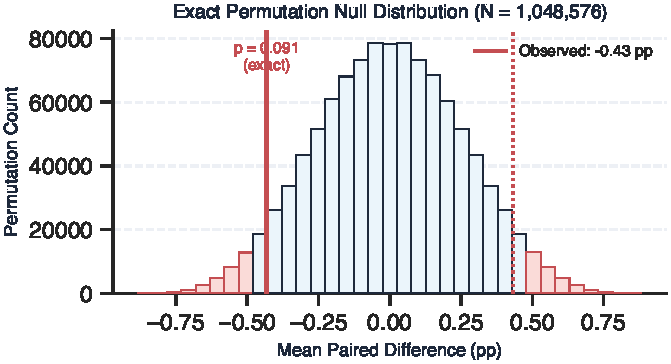
\includegraphics[width=0.62\linewidth]{figures/figure_cifar_permutation_null.pdf}
\caption{\textbf{Exact Paired Permutation Null Distribution on CIFAR-100 ($N = 20$).} Complete enumeration of all $2^{20} = 1{,}048{,}576$ sign-flip permutations for the primary contrast $\Delta_{\mathrm{total}} = S_1 - C_0$. The observed test statistic ($-0.43$ pp, solid red line) falls within the non-rejection region (exact two-tailed $p = 0.091$, shaded red tails).}\label{fig:supp_permutation_null}
\end{figure*}

\clearpage
\section{Multi-Domain Screening Spectrum and Goodness-of-Fit}\label{sec:supp_screening}

Table~\ref{tab:supp_screening_raw} lists seed-level measurements across the six multi-domain screening conditions evaluated on GroupNorm ResNet-18 across five random seeds per condition ($N = 30$ total runs). Table~\ref{tab:supp_spectrum_summary} provides the summarized condition-level statistics, and Table~\ref{tab:supp_screening_fits} evaluates parametric goodness-of-fit models.

\begin{table*}[!ht]
\caption{Seed-level measurements for the multi-domain screening spectrum across six conditions ($N = 5$ random seeds per condition, 30 runs total on GroupNorm ResNet-18).}\label{tab:supp_screening_raw}
\centering
\small
\resizebox{\linewidth}{!}{%
\begin{tabular}{l c cc c c cc cc}
\toprule
\textbf{Condition} & \textbf{Seed} & \textbf{Acc}($\vtheta_1$) & \textbf{Acc}($\vtheta_2$) & \textbf{Drop} (pp) & \textbf{Probe (\%)} & \textbf{Final Val (\%)} & \textbf{Final Test (\%)} & $\Dcka$ & $\urec$ \\
\midrule
\multirow{5}{*}{$B_0$ (Continuous)}
 & 42   & 53.64 & ---   & ---    & ---   & 57.38 & 56.69 & ---    & --- \\
 & 123  & 54.94 & ---   & ---    & ---   & 56.54 & 57.26 & ---    & --- \\
 & 456  & 52.78 & ---   & ---    & ---   & 55.52 & 56.44 & ---    & --- \\
 & 789  & 51.14 & ---   & ---    & ---   & 56.20 & 56.31 & ---    & --- \\
 & 2026 & 52.92 & ---   & ---    & ---   & 55.06 & 55.84 & ---    & --- \\
\midrule
\multirow{5}{*}{$B_1$ (Clean Reset)}
 & 42   & 53.64 & 60.08 & $-6.44$ & 67.72 & 58.40 & 58.06 & 0.2244 & 0 \\
 & 123  & 54.94 & 58.94 & $-4.00$ & 65.48 & 55.22 & 55.20 & 0.2086 & 0 \\
 & 456  & 52.78 & 58.32 & $-5.54$ & 65.82 & 56.14 & 57.38 & 0.2370 & 0 \\
 & 789  & 51.14 & 58.52 & $-7.38$ & 66.12 & 56.00 & 57.03 & 0.2237 & 0 \\
 & 2026 & 52.92 & 57.46 & $-4.54$ & 65.52 & 56.88 & 56.29 & 0.2054 & 0 \\
\midrule
\multirow{5}{*}{$B_3$ (CIFAR-10)}
 & 42   & 53.64 & 8.52  & 45.12  & 26.44 & 56.10 & 55.71 & 0.5642 & 2100 \\
 & 123  & 54.94 & 6.10  & 48.84  & 25.50 & 54.88 & 54.47 & 0.5462 & 3200 \\
 & 456  & 52.78 & 6.78  & 46.00  & 24.90 & 58.96 & 58.40 & 0.6135 & 3400 \\
 & 789  & 51.14 & 9.30  & 41.84  & 26.28 & 56.12 & 57.30 & 0.5539 & 1400 \\
 & 2026 & 52.92 & 8.70  & 44.22  & 26.72 & 54.22 & 54.05 & 0.5884 & 1900 \\
\midrule
\multirow{5}{*}{$B_4$ (STL-10)}
 & 42   & 53.64 & 8.18  & 45.46  & 23.12 & 55.22 & 56.14 & 0.6226 & 1500 \\
 & 123  & 54.94 & 5.86  & 49.08  & 21.18 & 58.70 & 59.25 & 0.6150 & 3100 \\
 & 456  & 52.78 & 7.58  & 45.20  & 21.06 & 54.78 & 55.45 & 0.6738 & 1700 \\
 & 789  & 51.14 & 6.38  & 44.76  & 21.50 & 58.30 & 58.33 & 0.6830 & 1400 \\
 & 2026 & 52.92 & 5.54  & 47.38  & 20.48 & 57.22 & 57.72 & 0.6800 & 3000 \\
\midrule
\multirow{5}{*}{$B_5$ (SVHN)}
 & 42   & 53.64 & 2.90  & 50.74  & 6.80  & 56.78 & 56.10 & 0.9030 & 5800 \\
 & 123  & 54.94 & 2.46  & 52.48  & 7.26  & 56.82 & 56.45 & 0.9160 & 9000 \\
 & 456  & 52.78 & 2.66  & 50.12  & 6.70  & 54.58 & 56.64 & 0.9161 & 4500 \\
 & 789  & 51.14 & 2.12  & 49.02  & 6.70  & 55.44 & 54.90 & 0.9115 & 4700 \\
 & 2026 & 52.92 & 2.78  & 50.14  & 7.34  & 56.84 & 56.44 & 0.9119 & 5300 \\
\midrule
\multirow{5}{*}{$B_7$ (Gaussian Noise)}
 & 42   & 53.64 & 1.30  & 52.34  & 5.10  & 54.12 & 54.14 & 0.9323 & 7800 \\
 & 123  & 54.94 & 1.20  & 53.74  & 4.78  & 51.04 & 51.26 & 0.9473 & 7800 \\
 & 456  & 52.78 & 1.72  & 51.06  & 4.12  & 54.84 & 56.16 & 0.9510 & 4700 \\
 & 789  & 51.14 & 1.66  & 49.48  & 4.06  & 55.66 & 56.04 & 0.9315 & 4000 \\
 & 2026 & 52.92 & 1.34  & 51.58  & 4.48  & 52.26 & 53.76 & 0.9046 & 9600 \\
\bottomrule
\end{tabular}%
}
\end{table*}

\begin{table*}[!ht]
\caption{Screening spectrum summary across the six experimental conditions ($N = 5$ seeds each, GroupNorm ResNet-18). Means are reported with sample standard deviations.}\label{tab:supp_spectrum_summary}
\centering
\small
\resizebox{\linewidth}{!}{%
\begin{tabular}{l ccccc c}
\toprule
\textbf{Condition} & $\Dcka$ & \textbf{Probe Drop (pp)} & \textbf{Target Drop (pp)} & \textbf{Final Val (\%)} & \textbf{Final Test (\%)} & $\urec$ \textbf{(Updates)} \\
\midrule
$B_0$ (Continuous Target) & --- & --- & --- & $56.14 \pm 0.93$ & $56.51 \pm 0.52$ & --- \\
$B_1$ (On-Target Reset)   & $0.2198 \pm 0.0116$ & $-5.58 \pm 1.34$ & $-5.58 \pm 1.34$ & $56.53 \pm 1.20$ & $56.79 \pm 1.09$ & $0 \pm 0$ \\
$B_3$ (CIFAR-10)          & $0.5732 \pm 0.0267$ & $45.20 \pm 2.65$ & $45.20 \pm 2.65$ & $56.06 \pm 1.77$ & $56.07 \pm 1.74$ & $2400 \pm 869$ \\
$B_4$ (STL-10)            & $0.6549 \pm 0.0336$ & $46.18 \pm 1.74$ & $46.18 \pm 1.74$ & $56.84 \pm 1.63$ & $57.38 \pm 1.54$ & $2140 \pm 826$ \\
$B_5$ (SVHN)              & $0.9117 \pm 0.0053$ & $50.50 \pm 1.27$ & $50.50 \pm 1.27$ & $56.09 \pm 1.06$ & $56.11 \pm 0.71$ & $5860 \pm 1828$ \\
$B_7$ (Gaussian Noise)    & $0.9334 \pm 0.0183$ & $51.64 \pm 1.57$ & $51.64 \pm 1.57$ & $53.58 \pm 1.87$ & $54.27 \pm 1.87$ & $6780 \pm 2350$ \\
\bottomrule
\end{tabular}%
}
\end{table*}

\begin{table*}[!ht]
\caption{Goodness-of-fit comparison for predictive models of auxiliary transfer performance across the screening spectrum. Lower AIC and BIC indicate superior model quality.}\label{tab:supp_screening_fits}
\centering
\small
\resizebox{\linewidth}{!}{%
\begin{tabular}{llcccc}
\toprule
\textbf{Metric} & \textbf{Model} & $R^2$ & \textbf{Adj.} $R^2$ & \textbf{AIC} & \textbf{BIC} \\
\midrule
Null Model & Intercept Only & 0.0000 & 0.0000 & 100.8 & 102.2 \\
CKA Drift ($\Dcka$) & Linear & 0.0117 & $-0.0236$ & 102.4 & 105.3 \\
CKA Drift ($\Dcka$) & Quadratic & 0.0411 & $-0.0299$ & 103.5 & 107.7 \\
Target Accuracy Drop & Linear & 0.0437 & 0.0095 & 101.4 & 104.3 \\
Probe Accuracy Drop & Linear & 0.1692 & 0.1395 & 97.2  & 100.0 \\
Target Recovery Latency ($\urec$) & Linear & 0.8542 & 0.8490 & 48.6  & 51.4 \\
Target Recovery Latency ($\urec$) & Quadratic & 0.8853 & 0.8768 & 43.1  & 47.3 \\
\bottomrule
\end{tabular}%
}
\end{table*}

\clearpage
\section{Archival Ten-Seed Confirmatory Cohort Data}\label{sec:supp_historical}

Table~\ref{tab:supp_ten_seed_confirmatory} reports summary statistics and paired contrasts, while Table~\ref{tab:supp_appendix_historical_raw} provides per-seed measurements for the archival confirmatory replication conducted on GroupNorm ResNet-18 across $N = 10$ seeds (seeds 1001--1010; 40 runs total).

\begin{table*}[!ht]
\caption{Archival confirmatory replication across $N = 10$ fresh seeds (seeds 1001--1010, 40 total runs on GroupNorm ResNet-18). Performance metrics are expressed in percentage points (pp) relative to continuous baseline $B_0$. Non-parametric $95\%$ bootstrap confidence intervals (\texttt{Boot CI}) are computed from 10,000 percentile resamples; parametric $95\%$ paired Student's $t$-intervals (\texttt{Paired $t$-CI}) use critical multiplier $t_{0.975, 9} = 2.262$.}\label{tab:supp_ten_seed_confirmatory}
\centering
\small
\resizebox{\linewidth}{!}{%
\begin{tabular}{l c cccc ccc}
\toprule
& & \multicolumn{4}{c}{\textbf{Equal Total Updates ($\Delta_{\mathrm{total}}$, Val)}} & \multicolumn{3}{c}{\textbf{Terminal Test ($\Delta_{\mathrm{total}}$)}} \\
\cmidrule(lr){3-6} \cmidrule(lr){7-9}
\textbf{Condition} & $N$ & \textbf{Mean Diff.} & \textbf{95\% Boot CI} & $p_{\mathrm{paired}}$ & $d_z$ & \textbf{Mean Diff.} & \textbf{95\% Paired $t$-CI} & \textbf{95\% Boot CI} \\
\midrule
Clean Reset ($B_1$)       & 10 & $+0.75$ & [$-0.99$, $+2.46$] & $0.4337$ & $+0.26$ & $+0.97$ & [$-0.81$, $+2.74$] & [$-0.54$, $+2.37$] \\
STL-10 Transfer ($B_4$)   & 10 & $+0.76$ & [$-0.38$, $+1.91$] & $0.2491$ & $+0.39$ & $+0.44$ & [$-0.93$, $+1.81$] & [$-0.63$, $+1.61$] \\
Gaussian Noise ($B_7$)    & 10 & $-2.99$ & [$-4.67$, $-1.55$] & $0.0059$ & $-1.13$ & $-2.81$ & [$-4.80$, $-0.82$] & [$-4.56$, $-1.22$] \\
\midrule
\multicolumn{9}{l}{\textbf{Paired Contrast: Auxiliary Transfer ($B_4$) vs. Clean Optimizer Reset ($B_1$)}} \\
$\bm{B_4 - B_1}$          & 10 & $+0.00$ & [$-1.04$, $+1.22$] & $0.9949$ & $+0.00$ & $\bm{-0.53}$ & [$\bm{-1.74}$, $\bm{+0.68}$] & [$\bm{-1.48}$, $\bm{+0.52}$] \\
\bottomrule
\end{tabular}%
}
\end{table*}

\begin{table*}[!ht]
\caption{Seed-level measurements for the archival ten-seed confirmatory cohort across four conditions ($N = 10$ seeds, 40 total runs on GroupNorm ResNet-18).}\label{tab:supp_appendix_historical_raw}
\centering
\small
\resizebox{\linewidth}{!}{%
\begin{tabular}{l c cc c c cc cc}
\toprule
\textbf{Condition} & \textbf{Seed} & \textbf{Acc}($\vtheta_1$) & \textbf{Acc}($\vtheta_2$) & \textbf{Probe}($\vtheta_2$) & \textbf{Val}($\vtheta_3$) & \textbf{Test}($\vtheta_3$) & \textbf{Probe}($\vtheta_3$) & \textbf{EffRank}($\vtheta_2$) & \textbf{EffRank}($\vtheta_3$) \\
\midrule
\multirow{10}{*}{$B_0$ (Continuous)}
 & 1001 & 51.90 & --- & --- & 56.30 & 55.80 & 64.12 & --- & 170.4 \\
 & 1002 & 51.58 & --- & --- & 56.38 & 56.10 & 63.48 & --- & 152.8 \\
 & 1003 & 52.04 & --- & --- & 54.06 & 55.16 & 61.96 & --- & 147.7 \\
 & 1004 & 53.38 & --- & --- & 55.56 & 56.73 & 62.04 & --- & 165.4 \\
 & 1005 & 52.96 & --- & --- & 55.26 & 54.78 & 62.26 & --- & 168.3 \\
 & 1006 & 51.78 & --- & --- & 52.66 & 53.35 & 62.12 & --- & 160.9 \\
 & 1007 & 53.74 & --- & --- & 55.06 & 55.71 & 62.08 & --- & 162.8 \\
 & 1008 & 53.98 & --- & --- & 55.66 & 56.91 & 62.68 & --- & 152.8 \\
 & 1009 & 51.96 & --- & --- & 56.50 & 55.65 & 62.38 & --- & 172.6 \\
 & 1010 & 54.54 & --- & --- & 58.88 & 59.88 & 64.50 & --- & 150.2 \\
\midrule
\multirow{10}{*}{$B_1$ (Clean Reset)}
 & 1001 & 51.90 & 54.76 & 61.18 & 57.94 & 57.60 & 63.52 & 174.8 & 168.9 \\
 & 1002 & 51.58 & 54.04 & 62.06 & 55.76 & 57.44 & 62.84 & 157.2 & 152.1 \\
 & 1003 & 52.04 & 54.10 & 61.30 & 57.34 & 57.78 & 63.42 & 152.3 & 149.0 \\
 & 1004 & 53.38 & 52.12 & 60.76 & 58.42 & 57.75 & 64.08 & 167.1 & 163.6 \\
 & 1005 & 52.96 & 54.20 & 61.40 & 55.08 & 56.01 & 62.52 & 172.3 & 168.6 \\
 & 1006 & 51.78 & 53.62 & 59.16 & 57.52 & 58.01 & 63.54 & 166.9 & 160.5 \\
 & 1007 & 53.74 & 53.76 & 59.64 & 58.36 & 58.91 & 63.62 & 168.8 & 160.5 \\
 & 1008 & 53.98 & 52.68 & 60.06 & 53.56 & 54.85 & 60.44 & 154.7 & 150.7 \\
 & 1009 & 51.96 & 55.98 & 61.32 & 52.12 & 51.91 & 61.06 & 176.6 & 170.1 \\
 & 1010 & 54.54 & 52.02 & 61.06 & 57.74 & 59.50 & 63.58 & 150.7 & 148.4 \\
\midrule
\multirow{10}{*}{$B_4$ (STL-10)}
 & 1001 & 51.90 & 6.98  & 21.44 & 57.26 & 55.48 & 63.42 & 127.1 & 156.0 \\
 & 1002 & 51.58 & 6.62  & 20.00 & 55.68 & 56.42 & 61.78 & 119.1 & 147.1 \\
 & 1003 & 52.04 & 7.84  & 22.88 & 56.34 & 56.46 & 63.96 & 113.7 & 140.1 \\
 & 1004 & 53.38 & 6.84  & 23.60 & 56.64 & 56.00 & 62.50 & 125.9 & 156.2 \\
 & 1005 & 52.96 & 6.58  & 21.68 & 57.08 & 56.98 & 62.22 & 127.4 & 160.4 \\
 & 1006 & 51.78 & 6.60  & 22.10 & 57.10 & 57.70 & 62.50 & 125.9 & 151.0 \\
 & 1007 & 53.74 & 6.66  & 20.78 & 56.22 & 56.90 & 64.16 & 122.2 & 150.2 \\
 & 1008 & 53.98 & 6.80  & 21.92 & 55.38 & 56.68 & 61.58 & 118.9 & 142.6 \\
 & 1009 & 51.96 & 6.72  & 22.40 & 55.96 & 54.31 & 62.90 & 128.3 & 162.2 \\
 & 1010 & 54.54 & 7.22  & 22.28 & 56.22 & 57.52 & 62.42 & 111.7 & 140.7 \\
\bottomrule
\end{tabular}%
}
\end{table*}

\clearpage
\section{Compact Vision Transformer (CViT) Architecture and Seed Data}\label{sec:supp_vit}

To evaluate whether findings generalize beyond convolutional inductive biases, we evaluate a Compact Vision Transformer (CViT). The CViT operates on non-overlapping $4 \times 4$ patches with embedding dimension $d = 256$, 8 transformer blocks, 8 attention heads, and MLP expansion factor 2, followed by Layer Normalization and mean pooling.

\begin{table*}[!ht]
\caption{Confirmatory comparison of Compact Vision Transformer (CViT) models across $N = 5$ random seeds (seeds 3001--3005, 15 total runs). Contrasts use two-sided paired Student's $t$-tests with Bonferroni-adjusted $\alpha_{\mathrm{adj}} = 0.025$.}\label{tab:supp_vit_summary}
\centering
\small
\resizebox{\linewidth}{!}{%
\begin{tabular}{l ccccc c}
\toprule
\textbf{Contrast Estimand} & \textbf{Mean Diff. (pp)} & \textbf{Paired SD} & \textbf{95\% Paired $t$-CI} & $t(4)$ & $p$-value & $d_z$ \\
\midrule
Detour vs. Continuous ($B_4 - B_0$) & $-0.06$ & 0.49 & [$-0.67$, $+0.55$] & $-0.26$ & 0.806 & $-0.12$ \\
Clean Reset vs. Continuous ($B_1 - B_0$) & $+0.21$ & 0.38 & [$-0.26$, $+0.68$] & $+1.23$ & 0.286 & $+0.55$ \\
Detour vs. Clean Reset ($B_4 - B_1$) & $-0.27$ & 0.44 & [$-0.81$, $+0.28$] & $-1.37$ & 0.244 & $-0.61$ \\
\bottomrule
\end{tabular}%
}
\end{table*}

\begin{table*}[!ht]
\caption{Seed-level measurements for the Compact Vision Transformer (CViT) evaluation across five independent random seeds (seeds 3001--3005, 15 total runs).}\label{tab:supp_vit_raw}
\centering
\small
\resizebox{\linewidth}{!}{%
\begin{tabular}{l c cc c c cc cc}
\toprule
\textbf{Condition} & \textbf{Seed} & \textbf{Acc}($\vtheta_1$) & \textbf{Acc}($\vtheta_2$) & \textbf{Probe}($\vtheta_2$) & \textbf{Val}($\vtheta_3$) & \textbf{Test}($\vtheta_3$) & \textbf{Probe}($\vtheta_3$) & \textbf{EffRank}($\vtheta_2$) & \textbf{EffRank}($\vtheta_3$) \\
\midrule
\multirow{5}{*}{$B_0$ (Continuous)}
 & 3001 & 42.44 & --- & --- & 44.62 & 45.43 & 47.78 & --- & 164.6 \\
 & 3002 & 42.62 & --- & --- & 42.76 & 43.20 & 45.90 & --- & 165.2 \\
 & 3003 & 41.22 & --- & --- & 41.44 & 43.05 & 44.86 & --- & 164.6 \\
 & 3004 & 38.84 & --- & --- & 39.98 & 40.55 & 41.88 & --- & 165.4 \\
 & 3005 & 43.10 & --- & --- & 43.16 & 44.42 & 46.46 & --- & 164.6 \\
\midrule
\multirow{5}{*}{$B_1$ (Clean Reset)}
 & 3001 & 42.44 & 42.26 & 44.92 & 43.58 & 44.97 & 46.96 & 156.1 & 165.0 \\
 & 3002 & 42.62 & 41.66 & 44.52 & 43.58 & 44.09 & 46.28 & 155.2 & 164.6 \\
 & 3003 & 41.22 & 41.22 & 43.76 & 43.42 & 43.57 & 46.24 & 156.0 & 165.2 \\
 & 3004 & 38.84 & 38.56 & 41.08 & 39.58 & 41.00 & 42.28 & 155.5 & 164.6 \\
 & 3005 & 43.10 & 43.44 & 45.98 & 43.36 & 44.90 & 46.54 & 155.4 & 164.4 \\
\midrule
\multirow{5}{*}{$B_4$ (STL-10)}
 & 3001 & 42.44 & 15.44 & 31.64 & 44.46 & 45.14 & 46.70 & 139.3 & 163.3 \\
 & 3002 & 42.62 & 15.24 & 31.52 & 43.60 & 44.05 & 47.06 & 136.8 & 163.5 \\
 & 3003 & 41.22 & 13.88 & 30.42 & 42.36 & 44.34 & 45.44 & 140.1 & 164.1 \\
 & 3004 & 38.84 & 12.16 & 28.24 & 40.36 & 40.79 & 42.26 & 137.6 & 163.8 \\
 & 3005 & 43.10 & 17.04 & 32.46 & 44.66 & 44.54 & 46.78 & 138.1 & 163.4 \\
\bottomrule
\end{tabular}%
}
\end{table*}

\clearpage
\section{Seed-Level Data for the \texorpdfstring{$2 \times 2$}{2x2} Factorial Decomposition}\label{sec:supp_factorial}

Table~\ref{tab:supp_factorial_raw} lists seed-level test classification accuracies across the six paired seeds ($s \in \{920001, \dots, 920006\}$) evaluated in the $2 \times 2$ factorial decomposition on CIFAR-100 under matched computational budgets ($35{,}000$ updates on GroupNorm ResNet-18). All arms fork from identical Phase 1 checkpoints $\theta_1^{(s)}$ at step 15,000.

\begin{table*}[!ht]
\caption{Seed-level test classification accuracies (\%) on CIFAR-100 across the six paired seeds (920001--920006) for the $2 \times 2$ factorial decomposition arms, alongside marginal effects and repeated-measures ANOVA statistics.}\label{tab:supp_factorial_raw}
\centering
\small
\resizebox{\linewidth}{!}{%
\begin{tabular}{l l l cccccc c}
\toprule
\textbf{Arm} & \textbf{Head Policy ($h$)} & \textbf{Momentum ($m$)} & \textbf{Seed 1} & \textbf{Seed 2} & \textbf{Seed 3} & \textbf{Seed 4} & \textbf{Seed 5} & \textbf{Seed 6} & \textbf{Mean $\pm$ SD} \\
\midrule
$F_{00}$ ($C_0$) & Retained target $h_A$ & Continuous carryover & 55.38 & 57.19 & 57.98 & 55.85 & 56.52 & 55.01 & $56.32 \pm 1.13$ \\
$F_{01}$         & Retained target $h_A$ & Zeroed ($\bm{v} \leftarrow \mathbf{0}$) & 57.77 & 56.95 & 57.59 & 55.79 & 57.32 & 55.86 & $56.88 \pm 0.86$ \\
$F_{10}$         & Temp head $h_{\mathrm{temp}}$ & Continuous carryover & 55.47 & 54.01 & 55.84 & 52.73 & 53.87 & 53.34 & $54.21 \pm 1.21$ \\
$F_{11}$ ($C_3$) & Temp head $h_{\mathrm{temp}}$ & Zeroed ($\bm{v} \leftarrow \mathbf{0}$) & 56.71 & 54.13 & 53.67 & 53.40 & 55.97 & 54.86 & $54.79 \pm 1.32$ \\
\midrule
\multicolumn{10}{l}{\textbf{Repeated-Measures Factorial Effects ($5$ degrees of freedom):}} \\
\multicolumn{3}{l}{Main effect of head substitution ($\Delta_{\mathrm{head}}$)} & \multicolumn{4}{c}{$-2.10$ pp ($95\%$ CI: [$-3.18$, $-1.02$] pp)} & \multicolumn{3}{c}{$F(1, 5) = 24.95, p = 0.004$} \\
\multicolumn{3}{l}{Main effect of momentum clearing ($\Delta_{\mathrm{mom}}$)}   & \multicolumn{4}{c}{$+0.57$ pp ($95\%$ CI: [$-0.64$, $+1.77$] pp)} & \multicolumn{3}{c}{$F(1, 5) = 1.47, p = 0.279$} \\
\multicolumn{3}{l}{Factorial interaction ($\Delta_{\mathrm{interaction}}$)}      & \multicolumn{4}{c}{$+0.02$ pp ($95\%$ CI: [$-1.25$, $+1.29$] pp)} & \multicolumn{3}{c}{$F(1, 5) = 0.002, p = 0.967$} \\
\bottomrule
\end{tabular}%
}
\end{table*}

\clearpage
\section{Seed-Level Data for the Applied Vision Fine-Tuning Cohort (ISIC 2019)}\label{sec:supp_applied}

Table~\ref{tab:supp_applied_primary_raw} compiles complete seed-level diagnostic, representation, and classification measurements across the primary confirmatory cohort ($N = 8$ paired seeds, $s \in \{1001, \dots, 1008\}$). Table~\ref{tab:supp_applied_pilot_raw} and Table~\ref{tab:supp_applied_pilot_summary} compile the exploratory pilot benchmark ($N = 2$ seeds, $s \in \{900001, 900002\}$). Table~\ref{tab:supp_isic_class_split} documents the complete class distribution and partition methodology for the ISIC 2019 dataset.

\subsection{ISIC 2019 Dataset Partitioning and Leakage Controls}\label{subsec:supp_isic_split}
The ISIC 2019 dermoscopy dataset consists of 25,331 clinical images distributed across 8 diagnostic categories \cite{codella2018skin,tschandl2018ham10000}. To establish reproducible and leakage-free evaluation, images were partitioned into class-stratified train (80\%, 20,264 images), validation (10\%, 2,533 images), and held-out test (10\%, 2,534 images) partitions using deterministic random seed 42. Partition manifests were cryptographically sealed using SHA-256 hashes prior to running any fine-tuning experiments. The test partition was locked and evaluated strictly once at terminal checkpoint $\theta_3$. Internal representation trajectory tracking ($D_{\mathrm{CKA}}$ and Effective Rank) used a fixed, disjoint probe of 2,000 validation images sampled via seed 142. Table~\ref{tab:supp_isic_class_split} reports the exact sample breakdown per diagnostic category across partitions.

\begin{table*}[!ht]
\caption{Class-stratified partition distribution for the ISIC 2019 clinical dermoscopy dataset (25,331 images total; 8 diagnostic categories; seed 42).}\label{tab:supp_isic_class_split}
\centering
\small
\begin{tabular}{ll cccc}
\toprule
\textbf{Category} & \textbf{Full Diagnostic Description} & \textbf{Train (80\%)} & \textbf{Val (10\%)} & \textbf{Test (10\%)} & \textbf{Total} \\
\midrule
MEL  & Melanoma & 3,618 & 452 & 452 & 4,522 \\
NV   & Melanocytic Nevus & 10,300 & 1,288 & 1,287 & 12,875 \\
BCC  & Basal Cell Carcinoma & 2,658 & 332 & 333 & 3,323 \\
AK   & Actinic Keratosis & 694 & 87 & 86 & 867 \\
BKL  & Benign Keratosis & 2,099 & 262 & 263 & 2,624 \\
DF   & Dermatofibroma & 191 & 24 & 24 & 239 \\
VASC & Vascular Lesion & 202 & 25 & 26 & 253 \\
SCC  & Squamous Cell Carcinoma & 502 & 63 & 63 & 628 \\
\midrule
\textbf{Total} & \textbf{All Diagnostic Classes} & \textbf{20,264} & \textbf{2,533} & \textbf{2,534} & \textbf{25,331} \\
\bottomrule
\end{tabular}
\end{table*}

\begin{table*}[!ht]
\caption{Seed-level primary confirmatory evaluation metrics on ISIC 2019 across the eight independent paired seeds (1001--1008). All arms fork from identical Phase 1 checkpoints $\theta_1$ at step 5,000. Accuracies, contrasts, and balanced accuracies are reported in percentage points (pp).}\label{tab:supp_applied_primary_raw}
\centering
\small
\resizebox{\linewidth}{!}{%
\begin{tabular}{l ccc ccc ccc ccc}
\toprule
 & \multicolumn{3}{c}{\textbf{Terminal Top-1 Acc. (\%)}} & \multicolumn{3}{c}{\textbf{Paired Contrasts (pp)}} & \multicolumn{3}{c}{\textbf{Phase 2 EffRank (Step 7k)}} & \multicolumn{3}{c}{\textbf{Phase 2 CKA Drift ($D_{\mathrm{CKA}}$)}} \\
\cmidrule(lr){2-4} \cmidrule(lr){5-7} \cmidrule(lr){8-10} \cmidrule(lr){11-13}
\textbf{Seed} & $C_0$ (12k) & $C_3$ (12k) & $S_1$ (12k) & $C_3 - C_0$ & $S_1 - C_3$ & $S_1 - C_0$ & $C_0$ & $C_3$ & $S_1$ & $C_0$ & $C_3$ & $S_1$ \\
\midrule
1001 & 85.35 & 85.04 & 85.20 & $-0.32$ & $+0.16$ & $-0.16$ & 1153.3 & 1130.0 & 789.5 & 0.146 & 0.206 & 0.507 \\
1002 & 86.14 & 84.17 & 84.60 & $-1.97$ & $+0.43$ & $-1.54$ & 1146.6 & 1120.4 & 788.3 & 0.159 & 0.154 & 0.468 \\
1003 & 84.60 & 84.41 & 85.55 & $-0.20$ & $+1.14$ & $+0.95$ & 1142.5 & 1113.3 & 791.8 & 0.159 & 0.217 & 0.530 \\
1004 & 84.09 & 84.84 & 84.41 & $+0.75$ & $-0.43$ & $+0.32$ & 1164.4 & 1129.2 & 789.4 & 0.166 & 0.171 & 0.437 \\
1005 & 84.60 & 85.43 & 84.80 & $+0.83$ & $-0.63$ & $+0.20$ & 1141.9 & 1123.2 & 780.2 & 0.137 & 0.154 & 0.439 \\
1006 & 85.20 & 84.76 & 85.55 & $-0.43$ & $+0.79$ & $+0.36$ & 1142.9 & 1110.1 & 763.6 & 0.152 & 0.180 & 0.486 \\
1007 & 85.87 & 84.25 & 84.41 & $-1.62$ & $+0.16$ & $-1.46$ & 1145.0 & 1131.3 & 795.0 & 0.156 & 0.176 & 0.474 \\
1008 & 85.55 & 84.56 & 83.58 & $-0.99$ & $-0.99$ & $-1.97$ & 1138.5 & 1106.6 & 798.8 & 0.145 & 0.156 & 0.464 \\
\midrule
\textbf{Mean} & \textbf{85.18} & \textbf{84.68} & \textbf{84.76} & $\bm{-0.49}$ & $\bm{+0.08}$ & $\bm{-0.41}$ & \textbf{1146.9} & \textbf{1120.5} & \textbf{787.1} & \textbf{0.153} & \textbf{0.177} & \textbf{0.476} \\
\textbf{SD}   & 0.70  & 0.42  & 0.67  & 1.01  & 0.73  & 1.08  & 8.3   & 9.6   & 10.9  & 0.010 & 0.024 & 0.032 \\
\bottomrule
\end{tabular}%
}
\end{table*}

\begin{figure*}[!ht]
\centering
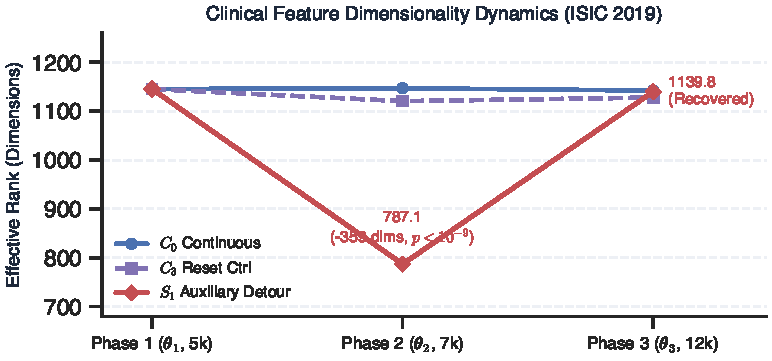
\includegraphics[width=0.62\linewidth]{figures/figure_applied_effrank_longitudinal.pdf}
\caption{\textbf{Longitudinal Effective Rank Trajectory in Clinical Dermoscopy.} Feature dimensionality dynamics across milestones $\bm{\theta}_1$ (step 5k warmup), $\bm{\theta}_2$ (step 7k post-detour), and $\bm{\theta}_3$ (step 12k terminal recovery). The off-task auxiliary detour ($S_1$, orange) triggers an acute drop of 359 dimensions at $\bm{\theta}_2$ ($t(7) = -53.4, p = 2.12 \times 10^{-10}$), which completely recovers to statistical parity with continuous baselines under subsequent target fine-tuning.}\label{fig:supp_applied_effrank}
\end{figure*}

\begin{figure*}[!ht]
\centering
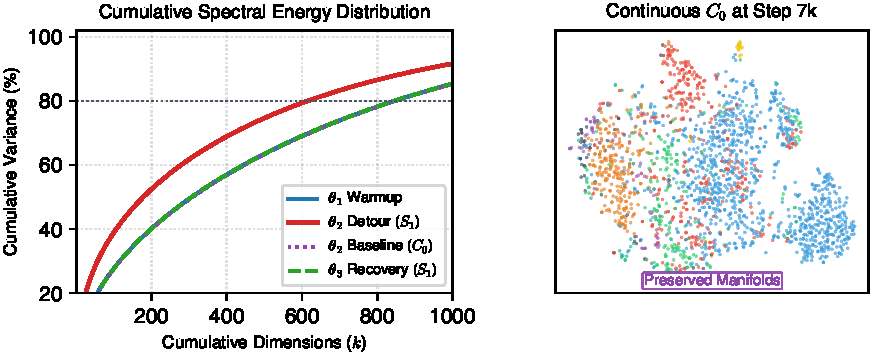
\includegraphics[width=0.82\linewidth]{figures/figure_applied_manifold_cumulative_and_c0.pdf}
\caption{\textbf{Supplementary Manifold Geometry Diagnostics on ISIC 2019.} (Left) Cumulative spectral energy distribution across singular value dimensions $k$, showing acute variance compression under the $S_1$ detour at $\bm{\theta}_2$ (red) compared to preserved variance in continuous training $C_0$ (purple). (Right) 2D t-SNE projection of clinical test lesions under uninterrupted training ($C_0$) at step 7k, demonstrating preserved diagnostic cluster structure.}\label{fig:supp_applied_manifold_cumulative}
\end{figure*}


\begin{table*}[!ht]
\caption{Applied fine-tuning pilot benchmark across $N = 2$ independent seeds (900001, 900002) on ISIC 2019 dermoscopy. Evaluates terminal metrics at $\theta_3$ (12,000 updates) alongside intermediate Phase 2 representation diagnostics at $\theta_2$ (7,000 updates).}\label{tab:supp_applied_pilot_summary}
\centering
\small
\resizebox{\linewidth}{!}{%
\begin{tabular}{ll cccc cc}
\toprule
\textbf{Condition} & \textbf{Phase 2 Description} & \textbf{Final Top-1 (\%)} & \textbf{Macro AUROC} & \textbf{Balanced Acc (\%)} & \textbf{ECE} & \textbf{Phase 2 EffRank} & \textbf{Phase 2 CKA Drift} \\
\midrule
$C_0$ & Continuous Target ISIC 2019 & $84.45 \pm 0.11$ & $0.9750 \pm 0.0026$ & $78.20 \pm 0.55$ & $0.1034 \pm 0.0023$ & $1151.5 \pm 8.9$ & $0.1841 \pm 0.0470$ \\
$C_3$ & On-Target Procedural Reset  & $85.27 \pm 0.56$ & $0.9767 \pm 0.0010$ & $77.68 \pm 0.64$ & $0.1002 \pm 0.0017$ & $1123.1 \pm 2.7$ & $0.2121 \pm 0.0589$ \\
$S_1$ & Auxiliary Detour (Imagenette) & $84.52 \pm 1.06$ & $0.9755 \pm 0.0014$ & $78.84 \pm 0.84$ & $0.0986 \pm 0.0050$ & $805.0 \pm 12.3$ & $0.4572 \pm 0.0146$ \\
$S_1\text{-shuf}$ & Shuffled Auxiliary Detour & $84.07 \pm 1.03$ & $0.9736 \pm 0.0037$ & $76.90 \pm 0.69$ & $0.0990 \pm 0.0120$ & $772.2 \pm 10.9$ & $0.4146 \pm 0.0213$ \\
\bottomrule
\end{tabular}%
}
\end{table*}

\begin{table*}[!ht]
\caption{Seed-level pilot benchmark evaluation metrics on ISIC 2019 across exploratory seeds 900001 and 900002.}\label{tab:supp_applied_pilot_raw}
\centering
\small
\resizebox{\linewidth}{!}{%
\begin{tabular}{l ccccc cccc}
\toprule
\textbf{Condition} & \textbf{Seed} & \textbf{Top-1 Acc. (\%)} & \textbf{Macro AUROC} & \textbf{Bal. Acc. (\%)} & \textbf{ECE} & \textbf{Brier Score} & \textbf{Phase 2 EffRank} & \textbf{Phase 2 $D_{\mathrm{CKA}}$} & \textbf{Phase 3 EffRank} \\
\midrule
$C_0$ (Continuous)        & 900001 & 84.52 & 0.9768 & 77.81 & 0.1050 & 0.2575 & 1145.2 & 0.1508 & 1139.8 \\
$C_3$ (Reset Ctrl)        & 900001 & 84.88 & 0.9760 & 78.13 & 0.1014 & 0.2482 & 1125.0 & 0.1705 & 1127.2 \\
$S_1$ (Auxiliary)         & 900001 & 83.77 & 0.9745 & 79.43 & 0.1022 & 0.2672 & 813.7  & 0.4469 & 1150.8 \\
$S_1\text{-shuf}$ (Shuf)  & 900001 & 83.34 & 0.9710 & 76.42 & 0.1075 & 0.2733 & 764.5  & 0.4297 & 1144.8 \\
\midrule
$C_0$ (Continuous)        & 900002 & 84.37 & 0.9731 & 78.59 & 0.1017 & 0.2531 & 1157.8 & 0.2173 & 1150.6 \\
$C_3$ (Reset Ctrl)        & 900002 & 85.67 & 0.9774 & 77.22 & 0.0990 & 0.2401 & 1121.2 & 0.2538 & 1122.2 \\
$S_1$ (Auxiliary)         & 900002 & 85.27 & 0.9765 & 78.24 & 0.0951 & 0.2443 & 796.3  & 0.4675 & 1144.2 \\
$S_1\text{-shuf}$ (Shuf)  & 900002 & 84.80 & 0.9763 & 77.39 & 0.0906 & 0.2458 & 779.9  & 0.3995 & 1133.5 \\
\bottomrule
\end{tabular}%
}
\end{table*}

\clearpage
\section{Leave-One-Condition-Out (LOCO) Recovery Prediction}\label{sec:supp_loco}

Table~\ref{tab:supp_loco_recovery_prediction} reports leave-one-condition-out cross-validation results evaluating whether representational geometric drift ($D_{\mathrm{CKA}}$) or task performance drop predicts recovery updates ($\urec$).

\begin{table*}[!ht]
\caption{Leave-one-condition-out cross-validation of recovery latency prediction across five intervention conditions ($B_1, B_3, B_4, B_5, B_7$). Performance is evaluated by Mean Absolute Error (MAE; updates) and Root Mean Squared Error (RMSE; updates).}\label{tab:supp_loco_recovery_prediction}
\centering
\small
\resizebox{\linewidth}{!}{%
\begin{tabular}{l cccc}
\toprule
& \multicolumn{2}{c}{\textbf{Unconstrained (All 5 Conditions)}} & \multicolumn{2}{c}{\textbf{Natural Distribution Shifts ($B_3, B_4, B_5$)}} \\
\cmidrule(lr){2-3} \cmidrule(lr){4-5}
\textbf{Predictor Metric} & \textbf{MAE (Updates)} & \textbf{RMSE (Updates)} & \textbf{MAE (Updates)} & \textbf{RMSE (Updates)} \\
\midrule
Linear CKA Drift ($\Dcka$)         & 1,646 & 2,059 & 2,230 & 2,367 \\
Target Accuracy Drop ($\Delta \mathrm{Acc}$) & 8,590 & 16,368 & 1,635 & 1,664 \\
Probe Accuracy Drop ($\Delta \mathrm{Probe}$) & 10,742 & 20,490 & 1,889 & 2,137 \\
\bottomrule
\end{tabular}%
}
\end{table*}

\end{document}
